%% ---------------------------------------------------------------------------
\documentclass[openany, twoside, a5paper, 10pt]{book}
%% ---------------------------------------------------------------------------
\usepackage[cp1251]{inputenc}
\usepackage[english,russian]{babel}
%% ---------------------------------------------------------------------------
\usepackage{indentfirst}
\frenchspacing
%% ---------------------------------------------------------------------------
\usepackage{url}
%% ---------------------------------------------------------------------------
\usepackage[dvips]{graphicx}
%\usepackage[pdftex]{graphicx}
%\usepackage{epstopdf}
%% ---------------------------------------------------------------------------
\usepackage{amsmath}
\usepackage{amssymb}
\usepackage{amscd}
\usepackage{bm}
\usepackage{ifmtarg}
%% ---------------------------------------------------------------------------
%\usepackage{soul}
%% ---------------------------------------------------------------------------
%\sloppy
%% ---------------------------------------------------------------------------
% a5paper: 148 x 210
% print area: 110 x 180
% top = bottom = (210 - 180) / 2 = 15
% left = right = (148 - 110) / 2 = 19
\usepackage[%
    left=1.9cm,%
    top=1.5cm,%
    right=1.9cm,%
    bottom=1.5cm,%
    headsep=0.2cm,%
    footskip=0.5cm,%
    includehead,%
    includefoot]{geometry}
%% ---------------------------------------------------------------------------
%% set lengthes
\newlength{\maxpicturewidth}
\setlength{\maxpicturewidth}{\textwidth }
\newlength{\maxpictureheight}
\setlength{\maxpictureheight}{\textheight }
%% ---------------------------------------------------------------------------
\usepackage{titlesec,titletoc}
%% ---------------------------------------------------------------------------
\setcounter{secnumdepth}{-1}
%% ---------------------------------------------------------------------------
\titleformat{\chapter}[display]
{\normalfont\huge\filcenter\bfseries}{}{20pt}{\Huge}
%% ---------------------------------------------------------------------------
\makeatletter
%% ---------------------------------------------------------------------------
% \Title[thanksto]{title}{name}{university}{city}{country}
\def\Title{%
    \@ifnextchar[{\TitleFootnote}{\TitleNoFootnote}
}
\newcounter{aster}
\setcounter{aster}{1}
%\renewcommand{\thefootnote}{\fnsymbol{footnote}}
\renewcommand{\thefootnote}{\fnsymbol{aster}}

\def\TitleFootnote[#1]#2#3#4#5#6{%
    \par
    \begin{centering}
        \medskip
        {\Large
         \textbf{#2}\@ifmtarg{#1}{}{\footnote{#1}}}\\
        \medskip
            #3\\
            \textit{#4, #5, #6}\\
        \smallskip
    \end{centering}
    \@afterheading
}
\def\TitleNoFootnote#1#2#3#4#5{%
    \par
    \begin{centering}
        \medskip
        {\Large
         \textbf{#1}}\\
        \medskip
            #2\\
            \textit{#3, #4, #5}\\
        \smallskip
    \end{centering}
    \@afterheading
}
%% ---------------------------------------------------------------------------
\newenvironment{references_rus}{%
    \par
    \medskip
    \centerline{\textbf{������ ����������}}
    \nopagebreak
    \medskip
    \@afterheading
    \begin{enumerate}
     \parsep=0pt plus 1pt
     \parskip=\parsep
     \itemsep=\parsep
}
{\end{enumerate}}
\newenvironment{references_eng}{%
    \par
    \medskip
    \centerline{\textbf{References}}
    \nopagebreak
    \medskip
    \@afterheading
    \begin{enumerate}
     \parsep=0pt plus 1pt
     \parskip=\parsep
     \itemsep=\parsep
}
{\end{enumerate}}
%% ---------------------------------------------------------------------------
\makeatother
%% ---------------------------------------------------------------------------

\begin{document}

%% ---------------------------------------------------------------------------
\renewcommand{\indexname}{Author index}
%% ---------------------------------------------------------------------------
%%%%%%%%%%%%%%%%% your_thesis_eng.tex %%%%%%%%%%%%%%%%%
%
% This is the template file for ORM 2016 proceedings.
%
% Please, fill in following the directions below.
%
%%%%%%%%%%%%%%%%%%%%%%%%%%%%%%%%%%%%%%%%%%%%%%%%%%%%%%%

\Title[%
% Insert here the acknowledgements of grants and/or any other
% information you wish to appear as a footnote, or leave this
% field blank.
This research is supported by\ldots%
]
{%
% Insert your title here
Title of your thesis%
}
{%
% Insert the authors' names here
B.B.~Baker, S.S.~Smith, and T.T.~Taylor%
}
{%
% Insert your institution here
Massachusetts Institute of Technology%
}
{%
% Insert your city here
Cambridge, MA%
}
{%
% Insert your country here
USA%
}

% Insert your thesis here.
% The entire submission should not exceed 3 pages if you plan a publication in conference proceedings.
%
% ATTENTION: Using 'thebibliography' environment is not allowed.
% Use 'references_eng' environment below to format the list of references.
% Please note that the latter environment does not provide automatic
% citation facilities. Cite manually using square brackets,
% e.g., [1], [2, 3], [4--6].
%
Your thesis. This work relies on the results in [1], and is an extension of the development in [2, 3].

% Insert your figure, if needed.
\begin{figure}[!h]
  \centering
  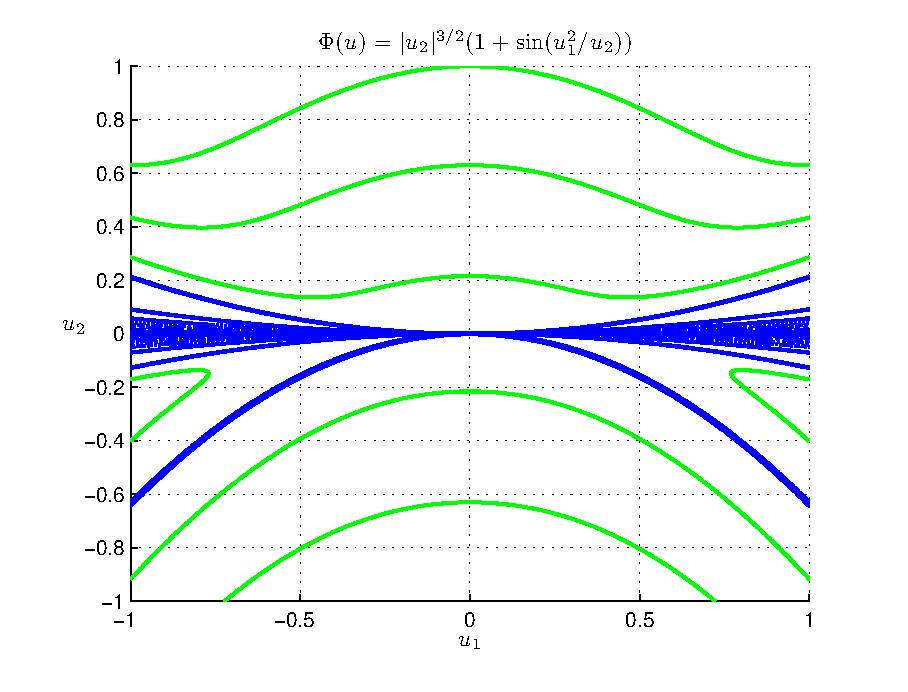
\includegraphics[width=0.7\maxpicturewidth]{your_figure.eps}
  \center{Fig.~1. Your caption.}
\end{figure}

\begin{references_eng}
% Insert your list of references here. The order of items in the list must
% agree with the order of their appearance in the text of your thesis.
% Use the '\url' command for citing url-s: e.g., \url{http://http://www.mathopt.org/}.

  \item % Reference No. 1
  Taylor~T.T. Article in a collection // Collection title. New York: Springer, 2012. P.~1--21.

  \item % Reference No. 2
  Smith~S.S. Book. New York: Springer, 2012.

  \item
  Baker~B.B. Journal article // Journal title. 2012. V.~1, \No ~1. P.~1--21.

% ...

\end{references_eng}

%%%%%%%%%%%%%%%%%%%%%%%%%%%%%%%%%%%%%%%%%%%%%%%%%%%%%%%

%\newpage
%\input{your_thesis_rus}
%% ---------------------------------------------------------------------------

\end{document}

%% ---------------------------------------------------------------------------

